\section{Introduction}
In this chapter we develop a joint model for TVWS spectrum sensing by incorporating frequency spectra gradients and time. The key insight is that static signals (such as TV transmission) will be sparse in time as the rarely change. We can make use of this by creating a model to detect ch ages in the signal across time. In this chapter we develop such a model, as a two-dimensional extension of the ideas of chapter \ref{chap:rect-basis}. 

To create a classification from measurements we develop a compressive and non-compressive method for estimating the joint model. The non-compressive model is a direct extension of ideas from chapter \ref{chap:rect-basis}, whilst the compressive method reduces a multi-time slot method to a single-time slot method.

We apply these methods to synthetic and real data (again supplied by OFCOM), and discuss the results.

\section{Time-Frequency Model}
In this section we extend the model from section \eqref{sec:sig-model}, to jointly estimate a collection of signals sensed over time. 

The rationale for this extension is that many signals are (approximately) constant over time, and thus exit an extra dimension of sparsity. Namely, when expanded in an appropriate basis a multi-time slot signal can be very sparse. This is because we need only sense changes from the underlying initial signal (e.g. a transmission turns on then off), as we assume that the underlying TV transmission is essentially constant.

In this case, we have a series frequency spectra \(\in \re^n\), sensed at \(T\) time instants. Consider a basis for \(\re^{n\times t}\) defined by the function:

\begin{definition}
\begin{equation}
l_{i,t}\left(x, \tau\right) = \mathbb{I}\left(t \leq \tau \right)\mathbb{I}\left(x \leq i\right)
\label{time-freq basis}
\end{equation}
\end{definition}

\begin{remark}
We can express these basis functions in terms of the basis functions \eqref{basis}, and similarly defined basis functions over time:

\begin{equation}
l_t\left(\tau\right) =
\begin{cases}
1 & \text{if } t \leq \tau \\
0 & \text{ otherwise } 
\end{cases}
\label{time-basis}
\end{equation}

That is, \(l_t\) is again a left-hand step function. 
\end{remark}

\begin{definition}[Tensor Product]
For two matrices \(A \in \re^{i \times j}\) and \(B \in \re^{k \times l}\) the tensor product is defined as:

\begin{equation}
A \kronecker B = \begin{pmatrix}
 a_{11} B & a_{12} B & \ldots & a_{1j} B \\
  a_{21} B & 1a_{22} B & \ldots & a_{2j} B\\
    \ldots  \\
     a_{i1} B & a_{i2} B & \ldots & a_{ij} B
\end{pmatrix}
\end{equation}

The resulting matrix has dimension \(ik \times jl\).

A useful property of tensor products is:

\begin{equation}
(A \kronecker B)(C \kronecker D) = AC \kronecker BD
\end{equation}

\end{definition}

\begin{proposition}
\begin{equation}
l_{i,t}\left(x, \tau\right) = l_i\left(x\right) \kronecker l_t\left(\tau\right)
\end{equation}
\begin{proof}
Consider a fixed frequency, w.l.o.g \(i=1\). Then 
\begin{equation}
l_{1,t}\left(x, \tau\right) = \mathbb{I}\left(x \leq 1\right)\mathbb{I}\left(t \leq \tau \right)
\end{equation}
There are \(T\) possible vectors, each of length \(n\), for this combination of \(\left(i,t\right)\). Therefore \(l_{1,t}\in \re^{1\times nT} \). As there are \(n\) possible frequency vectors, one for each fixed frequency basis function, we have \(n\times nT\) vectors. By symmetry of time and frequency, the same argument applies for a fixed time, and we have \(T\), \(1\times nT\) basis vectors in total, one for each fixed time instant. Therefore the joint time-frequency basis is in \(\re^{nT \times nT}\). As time and frequency are orthogonal in this representation, the proposition follows.
\end{proof}
\end{proposition}


Thus this basis can be represented with the following matrix in \(\re^{(nT)\times(nT)}\):

\begin{definition}
\begin{equation}
L = L_T \kronecker L_n
\label{def:time-freq matrix}
\end{equation}

where \(L_k\) is the matrix \eqref{lower-L} of size \(k \times k\). 
\end{definition}

\begin{lemma}
By direct computation, it follows that:

\begin{equation}
D = L^{-1} = L_T^{-1} \kronecker L_n^{-1} = D_T \kronecker D_n
\end{equation}

where \(D_k\) is the same as \eqref{inv-L}, and that:

\begin{align}
F &= LL^T \\
&= \left(L_n \kronecker L_T\right)\left(L_n \kronecker L_T\right)^T\\
&=L_TL_T^T \kronecker L_nL_n^T \\
&= F_T \kronecker F_n
\end{align}

where \(F_k\) is defined as in \eqref{def:Fmtx}.
\end{lemma}

We sense the frequency spectrum at \(T\) instants, collecting signals \(g_1, \ldots g_\tau\). 

similarly to \ref{basis-expansion} we model the signal as a linear combination of basis vectors:

\begin{equation}
g = L^Ta = \left(L_T^T \kronecker L_n^T\right)a
\end{equation}

\begin{definition}
Given a collection of vectors, \(\{a\}_{t=1}^T\), we write
\begin{equation}
a = \mathrm{vec}\left(a_t\right) = \sum_{t=1}^T e_t \kronecker a_t
\end{equation}
where \(e_t\) is the standard basis vector:

\begin{equation}
e_t =
\begin{cases}
1 & \text{if } t \leq T \\
0 & \text{ otherwise } 
\end{cases}
\end{equation}

\end{definition}

We can find an expression for \(a\) by taking the inner product of \(g\) with \(l_{j,s}\) (as \eqref{eq:h-est}):

\begin{align*}
h &= \langle g, l_{j,s}\left(x, \tau\right)\rangle \\
&= \sum_{i,t} g(x,\tau) \langle l_{i,t}, l_{j,s} \rangle \\
&= Fa
\end{align*}

The measurements in this model can be written as

\begin{equation}
y_T = A_Tg
\end{equation}

with 

\begin{equation}
A_T = I_T \kronecker A
\end{equation}

and \(A \sim N(0, 1/m)\).

\begin{proposition}
We can write the \(i^{th}\) column of the matrix \(L_k\) as, for \(k \leq j\):

\begin{equation}
L_k^T e_i = \sum_{j=1}^i e_j
\end{equation}

where \(e_j\) is the \(j^{th}\) canonical basis vector in \(\re^k\), with has a \(1\) in position \(j\) and is zeros everywhere else.

\begin{proof}
The \(i^{th}\) column of \(L_k\) will have \(i\) ones, and \(k-i\) zeros. It can be written in terms of the canonical basis \(e_j\), simply as sum up to the last \(1\) in position \(i\).
\end{proof}

\end{proposition}

In this case, we can write \(g\) as:

\begin{align*}
g = L^T a &= \left(L_T^T \kronecker L_n^T\right)\left(\sum_{t=1}^T e_t \kronecker a_t\right) \\
&= \sum_{t=1}^T L_T^T e_t \kronecker L_n^Ta_t \\
&= \sum_{t=1}^T \left(\sum_{j=1}^t e_j \right) \kronecker L_n^T a_t \\
&= \sum_{j=1}^T e_j \kronecker \sum_{t=j}^t L_n^T a_t \\
&= \sum_{j=1}^T e_j \kronecker b_j
\end{align*}

where we define \(b_j = \sum_{t=j}^T L_n^T a_t\). We can now write

\begin{align*}
y_T = A_Tg &= \left(I_T \kronecker A \right) \left(\sum_{j=1}^T e_i \kronecker b_j\right)\\
&= \sum_{j=1}^T e_j \kronecker Ab_j
\end{align*}

\begin{example}[Identical \(a_t\)]
Now consider the case where all the \(a_t\) are identical. In this case:

\begin{equation}
\twopartdef{a_T = a}{t=T}{a_t = 0}{t < T}
\end{equation}

so

\begin{equation}
b_j = \sum_{t=j}^T L_n^T a_t = L_n^T a = b
\end{equation}

Then

\begin{equation}
y_T = \left( \sum_{j=1}^T \right) \kronecker Ab = 1_T \kronecker Ab
\end{equation}
\end{example}

Let the \(s^{th}\) column of \(L_T^T\) be denoted by \(B_s\), then

\begin{align*}
\left(L_T^T\right)^{-1}B_s = D_T^T B_s = e_s
\end{align*}

As before, we form the estimator

\begin{align*}
\hat{h}_T = \sum_{i,t} \langle y_T, A_T l_{i,t} \rangle l_{i,t} \sim \frac{1}{mT} Fa
\end{align*}

Consider 

\begin{align*}
\langle y_T, A_T l_{i,t} \rangle &= \langle A_T^T y_T,l_{i,t} \rangle \\
&= \langle \left(I_T \kronecker A^T\right)\left(\sum_{j=1}^T e_j \kronecker Ab_j\right), \left(l_t \kronecker l_i\right)\rangle \\
&= \langle \sum_{j=1}^T e_j \kronecker A^TAb_j, \left(l_t \kronecker l_i\right)\rangle \\
&= \sum_{j=1}^T e_j^T l_t \kronecker b_j^TA^TAl_i \\
&\sim \frac{1}{m}\sum_{j=1}^T e_j^T l_t \kronecker b_j^Tl_i\\
&\stackrel{?}{=} \frac{1}{m}\sum_{j=1}^T j \kronecker F_n a
\end{align*}

where we used the expectation of a Wishart matrix between the \(5^{th}\) and \(6^{th}\) lines.


\subsection{Compressive Method}
\begin{definition}[Period-change vector]
Let
\begin{equation}
B = D \kronecker I_T
\end{equation}

then we define 

\begin{equation}
z = By
\end{equation}
\label{period vector}

This vector, identifies consecutive time slots in which the signal \(g\) is constant (i.e. does not change between sensing instants). As example, consider the following 5-slot signal:

\begin{figure}[h]
\centering
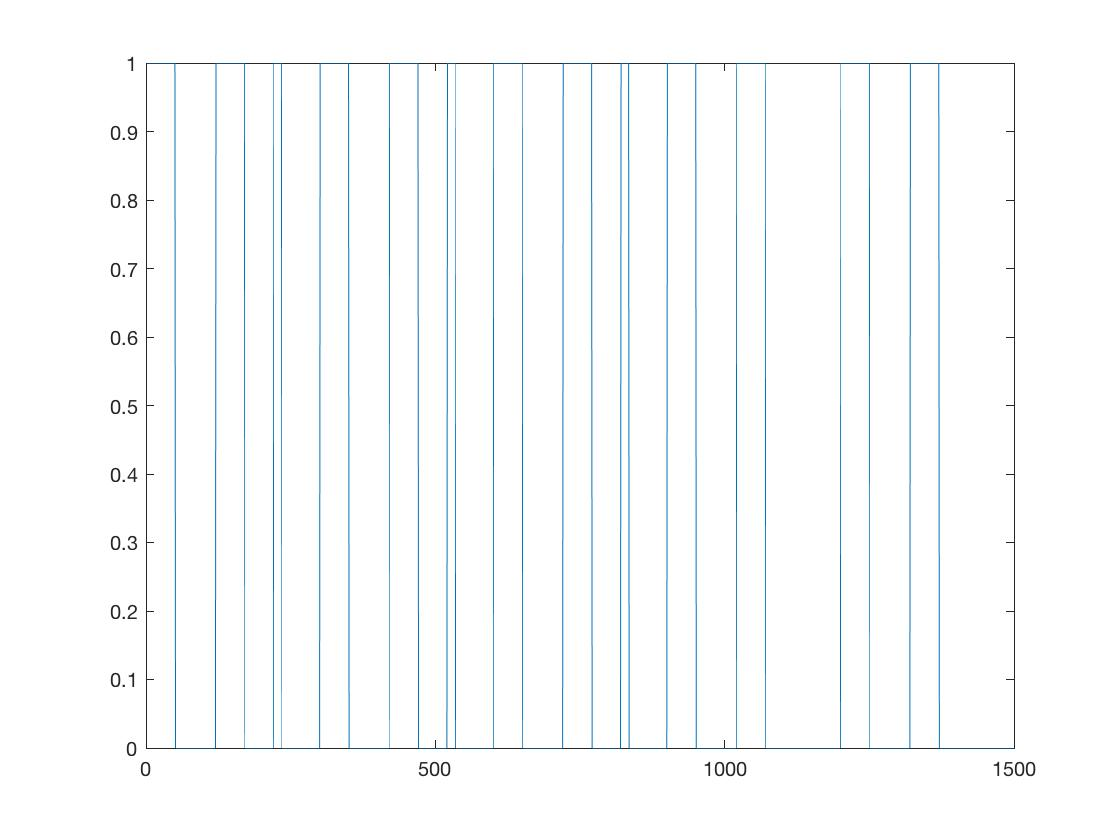
\includegraphics[height = 7.3 cm]{gt.jpg}
\caption{Example multiple time-slot signal}
\label{fig:gt}
\end{figure}

Whilst the compressive measurements of this signal are not revealing:

\begin{figure}[h]
\centering
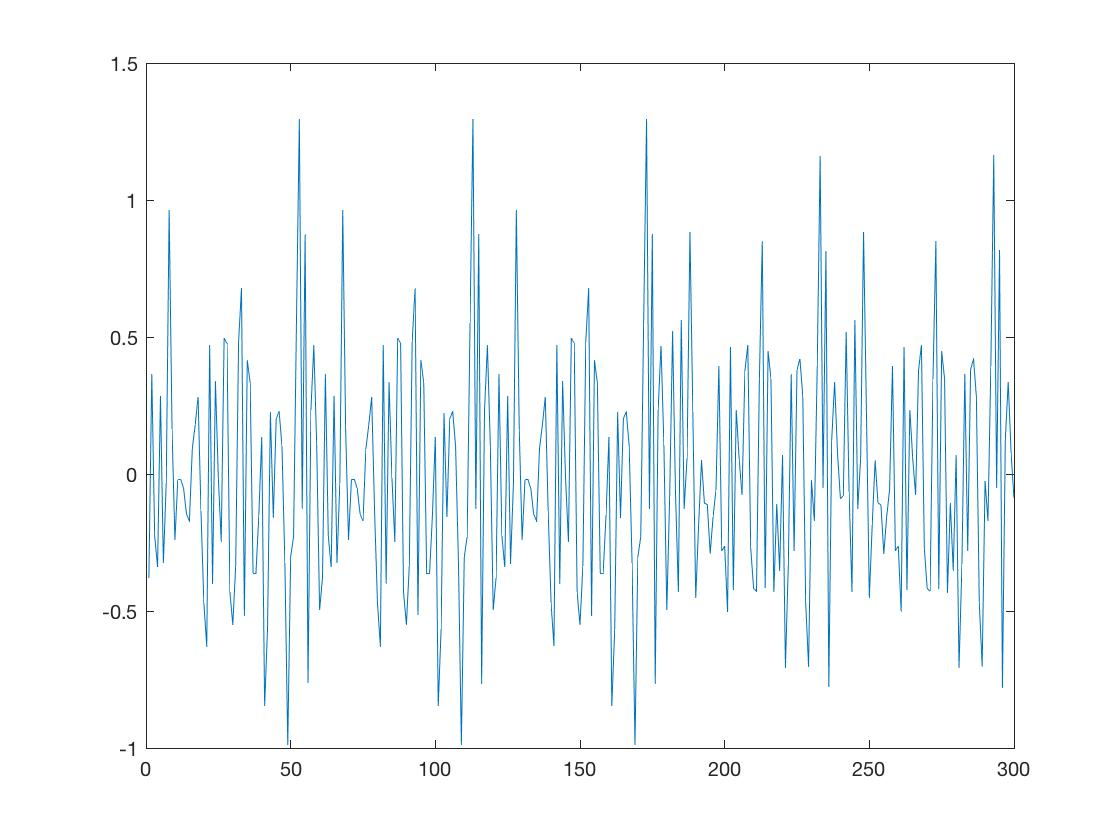
\includegraphics[height = 7.3 cm]{gt-compressed.jpg}
\caption{Compressive Measurements of the previous signal \ref{gt}}
\label{fig:ygt}
\end{figure}

The period change vector clearly identifies the periods where the original signal changes:

\begin{figure}[h]
\centering
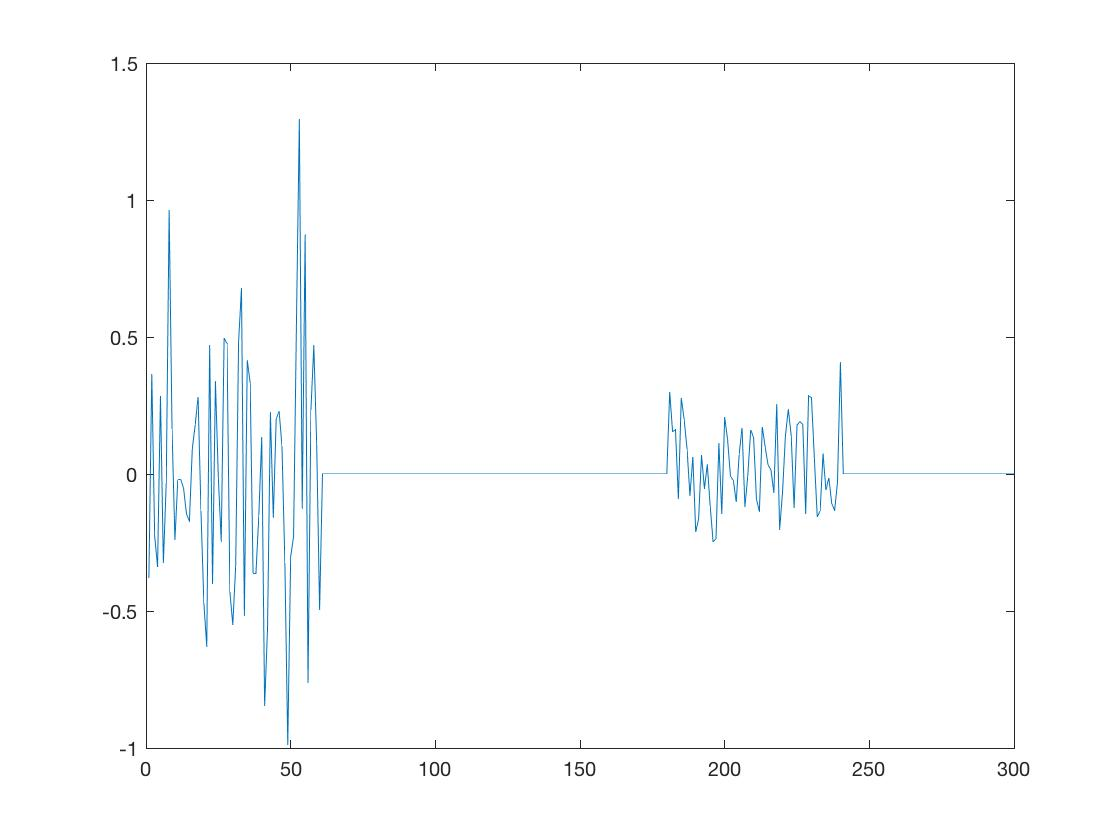
\includegraphics[height = 7.3 cm]{z-vec.jpg}
\caption{Period-change vector for the signal \ref{gt}}
\label{fig:period-vec}
\end{figure}

\end{definition}

We can use this vector to estimate a multiple time-slot signal. We use the following algorithm:

\begin{figure}
\begin{algorithmic}[1]
 %\SetAlgoLined % For previous releases [?]
 \Procedure{Estimate Occupancy Multiple Slot}{$y$, $A$, $k$}
 \State{A set compressive measurements \(y_T\), a measurement matrix \(A_T\), and an integer \(k\)}
 \State{\textbf{Returns}A estimate of the occupancy of a frequency spectrum, along multiple time slots.}
 \\
Compute \(z = By\) as per \eqref{period vector}
 \\
Count the number of zero consecutive parts of \(z\).
\\
For each group, take the mean of \(y_T\) for those \(t \in T\) belonging to that group, and use the procedure \ref{alg:single-slot} to form an estimate of those groups.
   	\EndProcedure
\end{algorithmic}
 \caption{Procedure for estimating occupancy of frequency spectra with multiple time slots}
 \label{alg:multiple-shot}
\end{figure}

\clearpage

\subsection{Non-compressive Method}
In this section we introduce a multi time-slot generalisation to the estimator \(h\) \eqref{eq:h-est}, adapted to the new basis.

\begin{definition}[Time-difference Vector]
We consider the estimator:
\begin{equation}
w = D^T A^T y
\end{equation}
\label{eq:w}
\end{definition}

\begin{remark}

We can see that this is an estimate of \(\alpha_T\) as:

\begin{align}
w &= D^T A^T y \\
&= D^T A^T A g_T \\
&=\left(D_T^T \kronecker D_n^T\right)\left(I_T \kronecker A_n^T\right)\left(I_T \kronecker A_n\right)g \\
\end{align}

\end{remark}

\begin{example}[Constant Signal]
i.e. the underlying signal remains constant over multiple time-slots.

We define the sensing matrix as:

\begin{equation}
A = I_T \kronecker A_n
\end{equation}

Thus we have

\begin{equation}
y = Ag = \mathrm{1}_T \kronecker A_n g_n
\end{equation}

and

\begin{align}
\alpha &= D^T g \\
&= \left(D_T^T \kronecker D_n^T \right)\left(I_T \kronecker g_n\right) \\
&=\left(D_T^T \kronecker D_n^T g_n\right) \\
&= e_T \kronecker \alpha_n
\end{align}

So, our estimator \eqref{eq:w} is, in this instance:

\begin{align}
w &= D^T A^T y \\
&= D^T A^T A g_T \\
&=\left(D_T^T \kronecker D_n^T\right)\left(I_T \kronecker A_n\right)\left(\mathrm{1}_T \kronecker A_n g_n\right) \\
&= e_T \kronecker \left(D_n^T A_n^T A_n L_n^T \alpha_n\right)\\
&\sim e_T \kronecker \left(D_n^T L_n^T \alpha_n\right)\\
&= e_T \kronecker \alpha_n \\
&= \alpha_T
\end{align}
\end{example}


\section{Results} \label{sec:results}

We now present some results for the multiple-stage algorithm \ref{alg:multiple-shot}.

\subsection{Synthetic Data}

\begin{figure}[h]
\centering
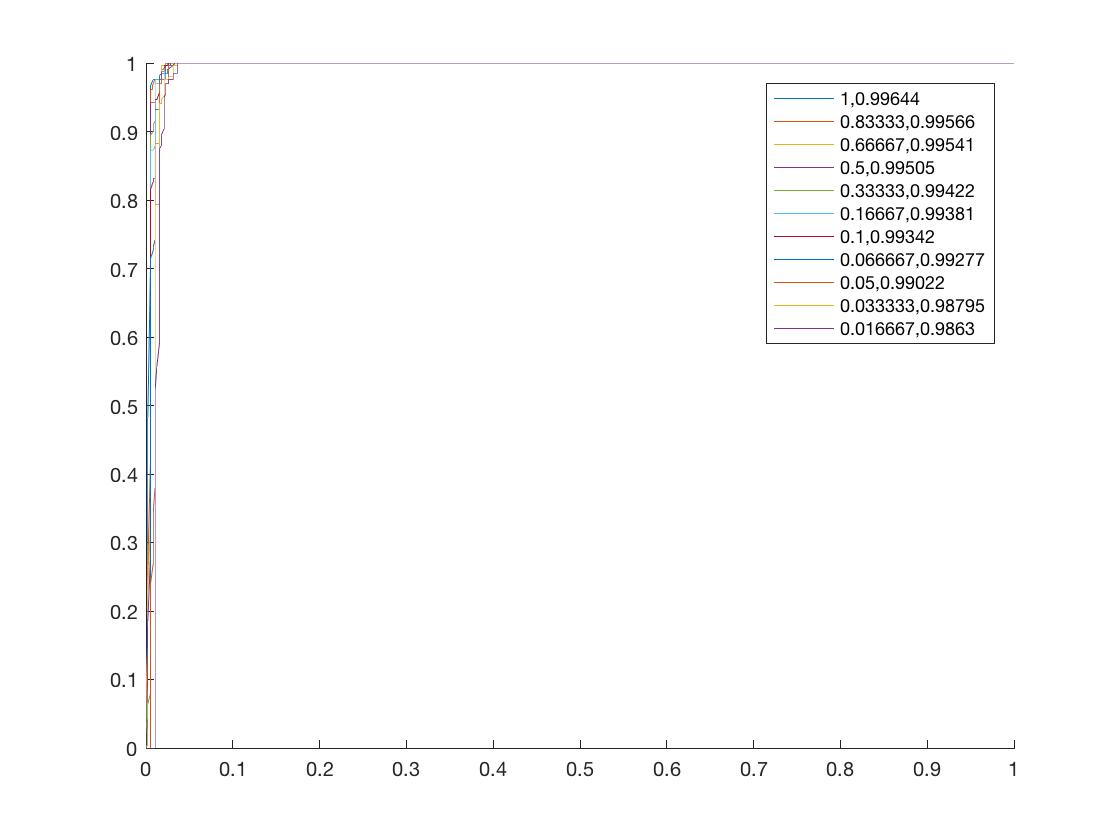
\includegraphics[height = 7.3 cm]{streaming-no-noise.jpg}
\caption{ROC curves for the multi-shot algorithm (as outlined in \ref{alg:multiple-slot}), for a signal in \(\re^{300}\), over 5 time slots. The first number in the legend is the ratio \(n/m\), whilst the second is the area under the curve. }
\label{multi_slot_different_k}
\end{figure}

In this instance the algorithm is able to provide an estimate, from only two groups i.e. it is able to infer that there is a change in the signal between the 3rd and 4th periods, and use this information to estimate the entire signal. 

\begin{figure}[h]
\centering
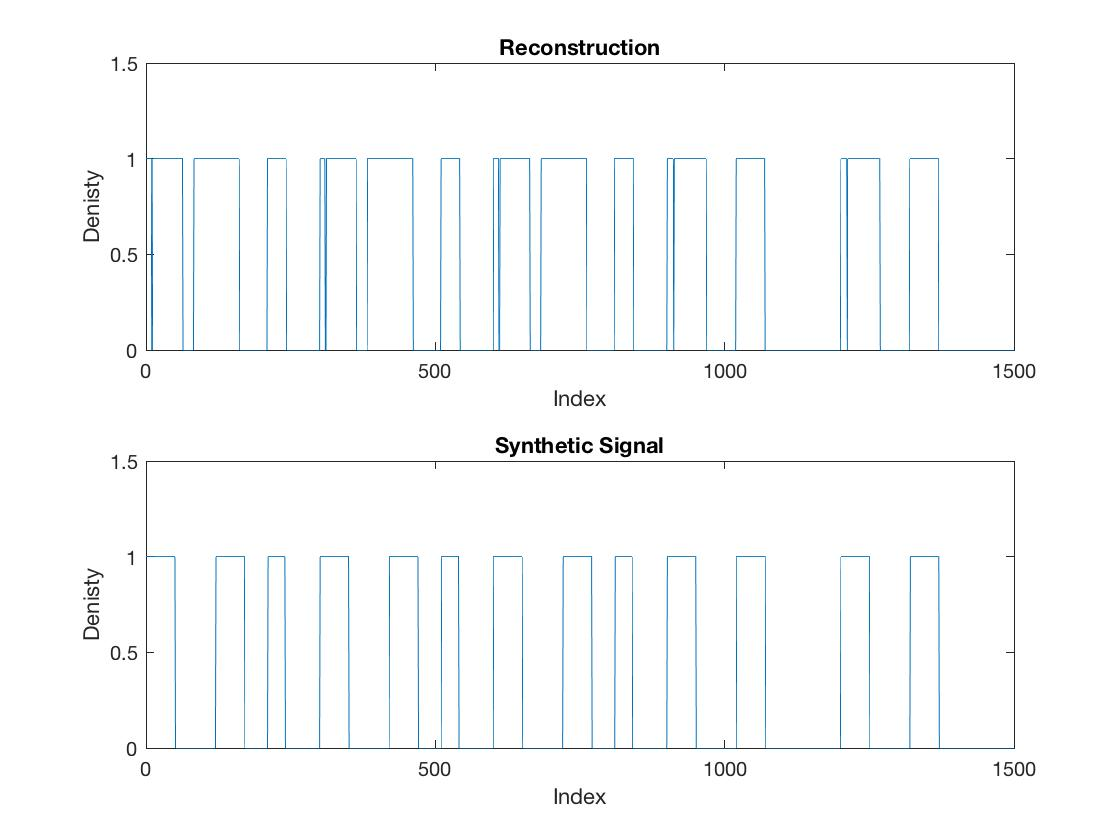
\includegraphics[height = 7.3 cm]{good_synthetic_multi_slot.jpg}
\caption{}
\label{good_sythetic_multi}
\end{figure}

\begin{figure}[h]
\centering
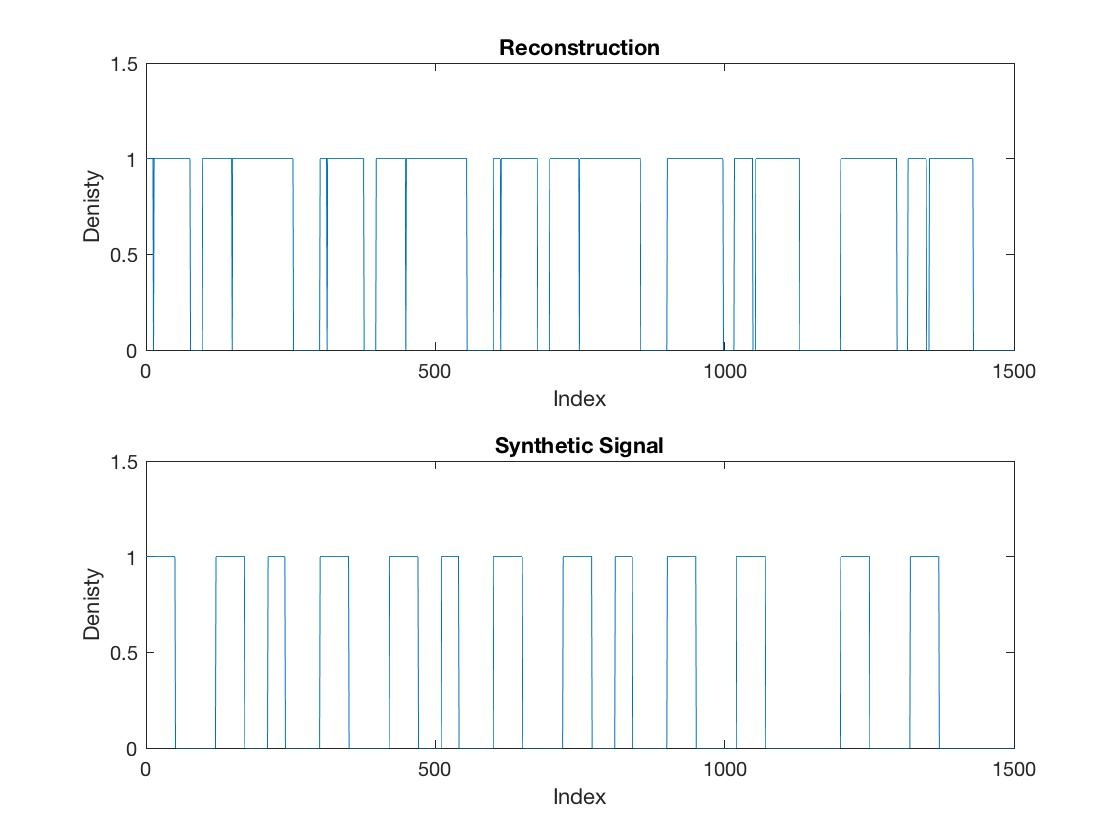
\includegraphics[height = 7.3 cm]{bad_synthetic_multi_slot.jpg}
\caption{}
\label{bad_synthetic_multi}
\end{figure}



\subsection{OFCOM Data}